We compare functional and identity adjacency on the same 1,935 low-history POIs with at least one NAICS-4 peer, using \(T=14\) and \(H=7\).
The December and January evaluations contain 297,990 and 338,625 scored events, respectively.
Target and neighbor evidence are classified using validation-period medians, before observing the test outcomes.
Table~\ref{tab:graph_transfer_summary} reports MAE gain within these evidence strata. Figure~\ref{fig:counterfactual_graph_transfer_map} resolves the pattern using validation-defined sextile cutpoints, with duplicate boundaries merged.

\begin{table}[!htbp]
\centering
\begingroup
\singlespacing
\fontsize{9pt}{10.5pt}\selectfont
\setlength{\tabcolsep}{4pt}
\renewcommand{\arraystretch}{1.08}
\caption{MAE gain over identity adjacency within validation-defined target/neighbor evidence strata at $T=14$, $H=7$. Values are means and standard deviations across five fitted seeds; positive values indicate lower error under functional adjacency.}
\label{tab:graph_transfer_summary}
\begin{adjustbox}{max width=\linewidth}
\begin{tabular}{lrrrr}
\toprule
Target / neighbor evidence & Dec. NAICS-2 & Dec. NAICS-4 & Jan. NAICS-2 & Jan. NAICS-4 \\
\midrule
Low / low & $-0.005\pm 0.004$ & $0.002\pm 0.006$ & $-0.012\pm 0.005$ & $0.001\pm 0.006$ \\
Low / high & $-0.056\pm 0.012$ & $-0.037\pm 0.007$ & $-0.191\pm 0.025$ & $-0.043\pm 0.007$ \\
High / low & $0.015\pm 0.009$ & $0.027\pm 0.014$ & $0.005\pm 0.007$ & $0.020\pm 0.011$ \\
High / high & $-0.032\pm 0.011$ & $-0.020\pm 0.010$ & $-0.118\pm 0.017$ & $-0.025\pm 0.009$ \\
\bottomrule
\end{tabular}
\end{adjustbox}
\endgroup
\end{table}


\begin{figure}[!htbp]
\centering
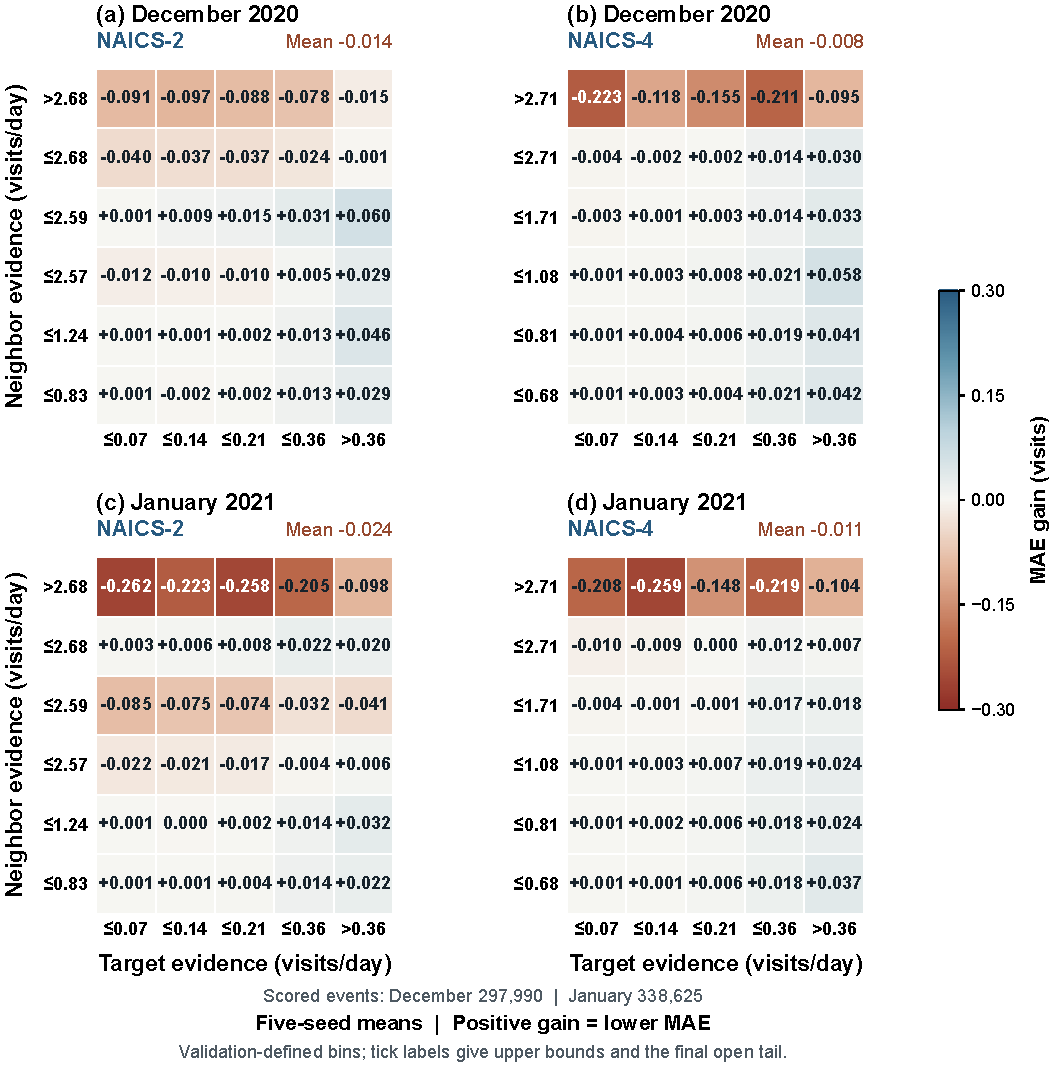
\includegraphics[width=\linewidth]{art/pre_outcome_graph_transfer.pdf}
\caption{Five-seed mean MAE gain over identity adjacency across target and neighbor evidence at \(T=14\), \(H=7\). Validation sextile cutpoints define the bins; ticks show successive upper bounds and the open tail. Positive gains indicate lower error under functional adjacency. Panel means weight cells by scored events; each cell contains at least 602 events. Fitted models and bin boundaries remain fixed in January.}
\label{fig:counterfactual_graph_transfer_map}
\end{figure}

Neighbor utility varies with both target evidence and neighbor activity.
For low target evidence and high neighbor evidence, NAICS-2 increases MAE by \(0.056\) visits in December and \(0.191\) in January; the corresponding increases under NAICS-4 are \(0.037\) and \(0.043\).
When target evidence is high and neighbor evidence is low, both graphs instead yield positive mean gains in both months.
Across all matched targets, NAICS-2 increases MAE by \(0.014\) in December, with a paired joint temporal--spatial 95\% interval of \([0.006,0.022]\), and by \(0.024\) in January, with an interval of \([0.013,0.037]\).
The corresponding NAICS-4 increases are \(0.008\) and \(0.011\); its December interval \([-0.001,0.017]\) includes zero.
These comparisons locate the largest errors in an evidence stratum that can be identified before the target visits are realized.

NAICS-4 and top category induce the same partition of the 9,884 POIs into 134 groups and therefore represent one graph specification.
NAICS-2 forms 22 groups, with a mean non-self degree of 1,586.5 compared with 767.0 under NAICS-4.
The clique comparison consequently changes both functional detail and neighborhood size.

Table~\ref{tab:semantic_granularity_transfer} holds the non-self degree fixed within each target. At $k=10$, NAICS-4 reduces December MAE relative to random neighbors by $0.0082$ for GraphGRU and $0.0056$ for Fixed-MTGNN, with joint temporal and 3-km spatial intervals of $[-0.0140,-0.0020]$ and $[-0.0069,-0.0044]$. The corresponding January reductions are $0.0126$ and $0.0037$. Relative to identity adjacency, however, GraphGRU error increases by $0.0645$ in December, while Fixed-MTGNN error decreases by $0.0080$. Functional similarity thus helps identify neighbors within a fixed-size graph, while the utility of graph propagation depends on the forecasting architecture.

\begin{table}[!htbp]
\centering
\begingroup
\singlespacing
\fontsize{9pt}{10.5pt}\selectfont
\setlength{\tabcolsep}{4pt}
\renewcommand{\arraystretch}{1.08}
\caption{Degree-controlled graph comparison at $T=14$, $H=7$. Each target has the same non-self degree under NAICS-2, NAICS-4, and random graphs, capped by $k$ and its available NAICS-4 peers. Values are five-seed MAE means and standard deviations.}
\label{tab:semantic_granularity_transfer}
\begin{adjustbox}{max width=\linewidth}
\begin{tabular}{llrrrrrr}
\toprule
Model & $k$ & Dec. NAICS-2 & Dec. NAICS-4 & Dec. random & Jan. NAICS-2 & Jan. NAICS-4 & Jan. random \\
\midrule
GraphGRU & 5 & $1.394\pm 0.002$ & $1.395\pm 0.012$ & $1.397\pm 0.001$ & $1.405\pm 0.001$ & $1.401\pm 0.012$ & $1.409\pm 0.003$ \\
GraphGRU & 10 & $1.375\pm 0.004$ & $1.366\pm 0.004$ & $1.374\pm 0.007$ & $1.387\pm 0.003$ & $1.375\pm 0.001$ & $1.388\pm 0.006$ \\
GraphGRU & 20 & $1.362\pm 0.006$ & $1.360\pm 0.006$ & $1.359\pm 0.010$ & $1.376\pm 0.008$ & $1.369\pm 0.007$ & $1.375\pm 0.011$ \\
\addlinespace[3pt]
Fixed-MTGNN & 5 & $1.226\pm 0.005$ & $1.223\pm 0.003$ & $1.226\pm 0.005$ & $1.250\pm 0.008$ & $1.246\pm 0.004$ & $1.247\pm 0.004$ \\
Fixed-MTGNN & 10 & $1.220\pm 0.005$ & $1.219\pm 0.005$ & $1.224\pm 0.006$ & $1.242\pm 0.007$ & $1.240\pm 0.008$ & $1.244\pm 0.007$ \\
Fixed-MTGNN & 20 & $1.224\pm 0.006$ & $1.221\pm 0.005$ & $1.224\pm 0.006$ & $1.247\pm 0.007$ & $1.242\pm 0.010$ & $1.247\pm 0.009$ \\
\bottomrule
\end{tabular}
\end{adjustbox}
\endgroup
\end{table}


The spatial and visit-correlation alternatives in Table~\ref{tab:spatial_graphs} show the same architectural distinction. All three GraphGRU alternatives have higher MAE than identity adjacency in both periods. Distance-neighbor propagation reduces Fixed-MTGNN MAE by $0.0051$ in December and $0.0045$ in January, with joint intervals of $[-0.0089,-0.0022]$ and $[-0.0071,-0.0020]$.

\begin{table}[!htbp]
\centering
\begingroup
\singlespacing
\fontsize{9pt}{10.5pt}\selectfont
\setlength{\tabcolsep}{4pt}
\renewcommand{\arraystretch}{1.08}
\caption{Additional fixed spatial and visit-correlation graphs at $T=14$, $H=7$. Values are five-seed MAE means and standard deviations.}
\label{tab:spatial_graphs}
\begin{adjustbox}{max width=\linewidth}
\begin{tabular}{llrr}
\toprule
Model & Adjacency & December & January \\
\midrule
GraphGRU & Distance KNN & $1.375\pm 0.010$ & $1.381\pm 0.009$ \\
GraphGRU & Distance RBF & $1.348\pm 0.011$ & $1.357\pm 0.010$ \\
GraphGRU & Visit correlation & $1.346\pm 0.010$ & $1.358\pm 0.011$ \\
Fixed-MTGNN & Distance KNN & $1.222\pm 0.008$ & $1.242\pm 0.009$ \\
\bottomrule
\end{tabular}
\end{adjustbox}
\endgroup
\end{table}


The outcome-conditioned transfer regimes remain descriptive assignments; in particular, negative MAE gain for a zero-visit event with positive graph lift follows directly from its definition.
